\section{Score Distributions at Epoch 5}

\begin{figure}[h]
\centering
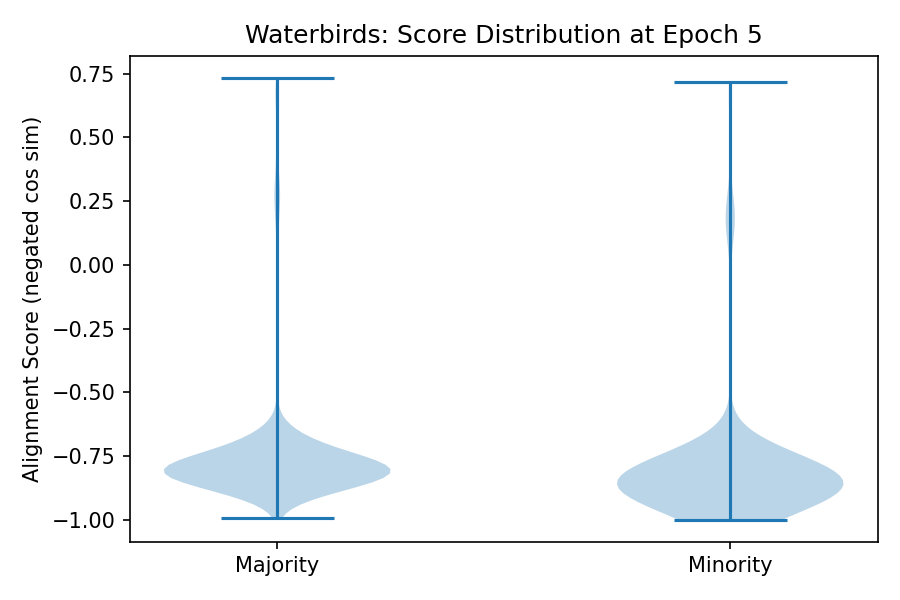
\includegraphics[width=0.85\linewidth]{figures/score_distribution_epoch5_waterbirds.png}
\caption{Alignment score ($a_i$) distributions by group on Waterbirds at epoch~5, overlaid kernel density estimates. Minority group distribution (landbird-on-water, waterbird-on-land) is shifted toward \emph{lower} $a_i$ values --- i.e., higher raw cosine similarity with the batch mean --- confirming the inversion: minority appears more aligned, not less. Loss distributions in the same figure show clean minority/majority separation.}
\label{fig:score_dist_wb}
\end{figure}

\begin{figure}[h]
\centering
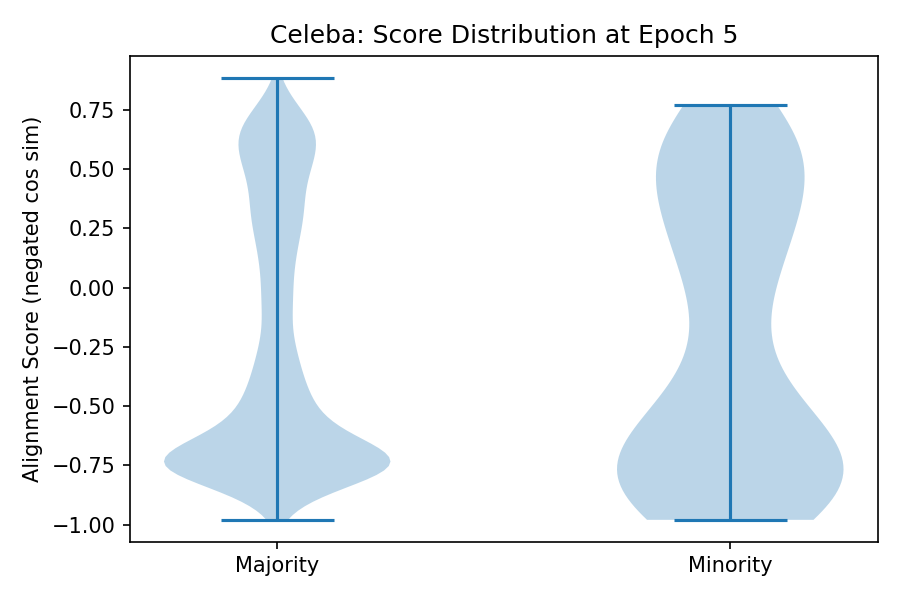
\includegraphics[width=0.85\linewidth]{figures/score_distribution_epoch5_celeba.png}
\caption{CelebA alignment score distributions at epoch~5 by group (blond-male minority vs.\ all others). Minority and majority distributions are near-identical under alignment score, confirming the signal is not discriminative. Loss distributions show clear separation (minority has higher loss).}
\label{fig:score_dist_celeba}
\end{figure}

\section{ROC Curves at Best Alignment Epoch}

\begin{figure}[h]
\centering
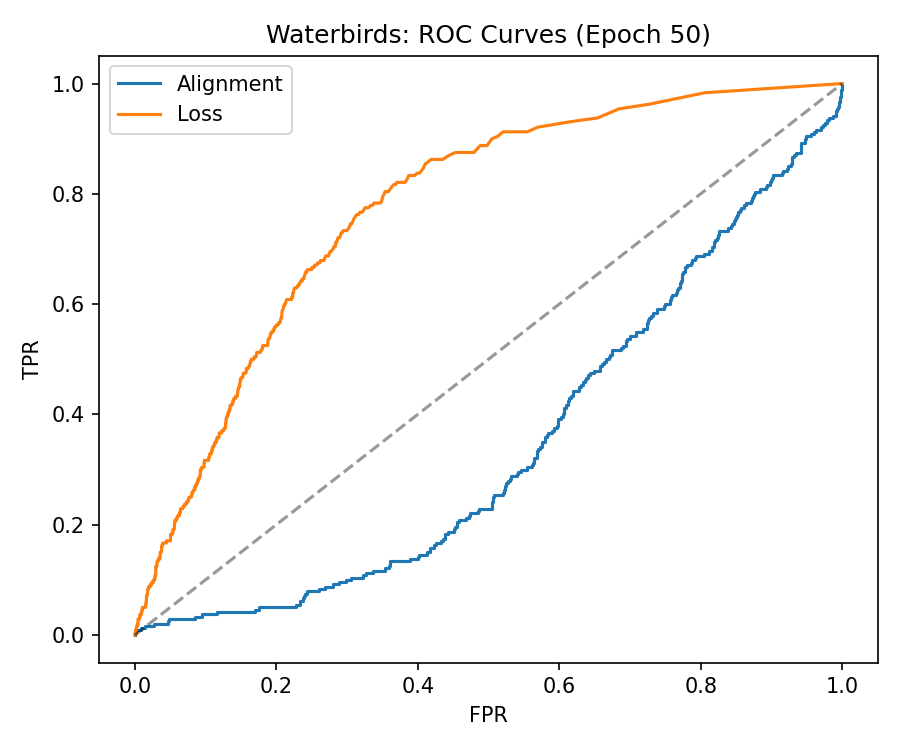
\includegraphics[width=0.85\linewidth]{figures/roc_curves_best_epoch_waterbirds.png}
\caption{ROC curves at epoch~50 (best alignment epoch on Waterbirds). Alignment ROC curve lies near the diagonal (AUC = 0.349); loss ROC curve shows substantial area above diagonal (AUC = 0.775).}
\label{fig:roc_wb}
\end{figure}

\begin{figure}[h]
\centering
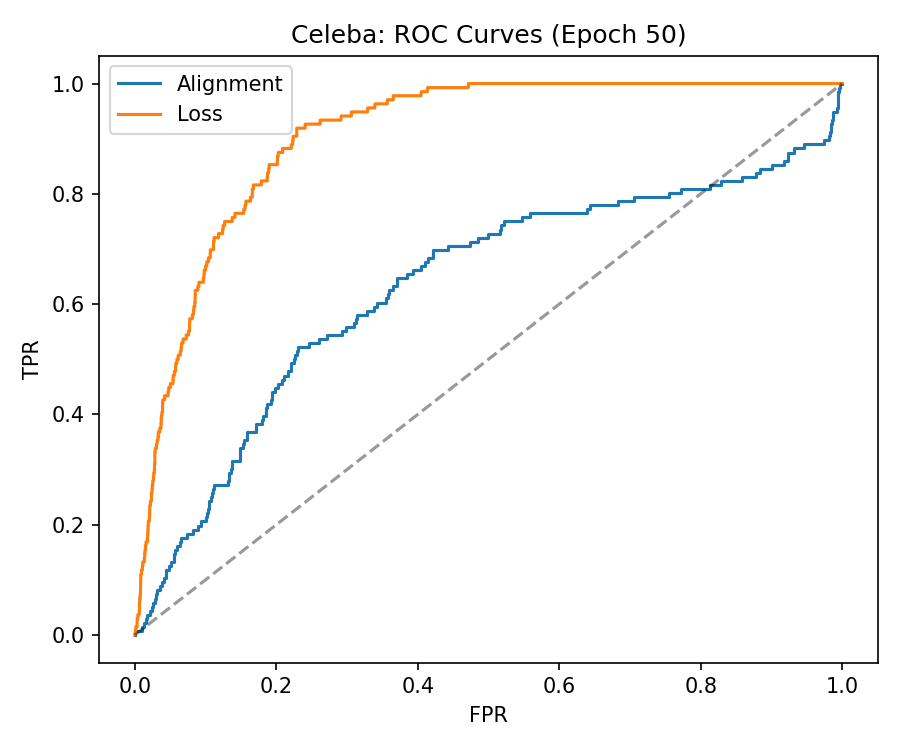
\includegraphics[width=0.85\linewidth]{figures/roc_curves_best_epoch_celeba.png}
\caption{ROC curves at epoch~50 (best alignment epoch on CelebA). Alignment shows slightly positive AUC (0.632) but well below loss (0.905).}
\label{fig:roc_celeba}
\end{figure}

\section{Experiment Configuration Details}

Full hyperparameter table, minority group ID encoding, and dataset preprocessing details are provided in Section~\ref{sec:methodology}.
Code is available at [anonymized for review].
